\documentclass{article}
\usepackage{setspace}
%\usepackage{subfigure}

\pagestyle{plain}
\usepackage{amssymb,graphicx,color}
\usepackage{amsfonts}
\usepackage{latexsym}
\usepackage{a4wide}
\usepackage{amsmath}
\usepackage{paper}
\usepackage{mathtools}

\newtheorem{theorem}{Theorem}
\newtheorem{lemma}[theorem]{Lemma}
\newtheorem{corollary}[theorem]{Corollary}
\newtheorem{proposition}[theorem]{Proposition}
\newtheorem{remark}[theorem]{Remark}
\newtheorem{definition}[theorem]{Definition}
\newtheorem{fact}[theorem]{Fact}

\newtheorem{problem}[theorem]{Problem}
\newtheorem{exercise}[theorem]{Exercise}
\def \set#1{\{#1\} }




\newenvironment{proof}{
PROOF:
\begin{quotation}}{
$\Box$ \end{quotation}}

\usepackage{xcolor}
\newcommand{\jk}[1]{{\color{blue} [JK: #1]}}
\newcommand{\jw}[1]{{\color{gray} [JW: #1]}}

\newcommand{\nats}{\mbox{\( \mathbb N \)}}
\newcommand{\rat}{\mbox{\(\mathbb Q\)}}
\newcommand{\rats}{\mbox{\(\mathbb Q\)}}
\newcommand{\reals}{\mbox{\(\mathbb R\)}}
\newcommand{\ints}{\mbox{\(\mathbb Z\)}}
\newcommand{\Cat}{\operatorname{\mathcal{C}}}
\newcommand{\Chol}{\operatorname{Chol}}
\newcommand{\KLD}{\operatorname{\mathbb{D}_{KL}}}
\newcommand{\D}{\operatorname{\mathbb{D}}}
\newcommand{\WD}{\operatorname{\mathbb{D}_{W_2}}}
\newcommand{\tr}{\operatorname{tr}}
\newcommand{\diag}{\operatorname{diag}}
\newcommand{\GP}{\operatorname{\mathcal{GP}}}

\DeclareMathOperator*{\argmax}{arg\,max}
\DeclareMathOperator*{\argmin}{arg\,min}

% make sure equation numbers start with the section they are from
\numberwithin{equation}{section}
%%%%%%%%%%%%%%%%%%%%%%%%%%


\title{  	{ 
\includegraphics[scale=.5]{ucl_logo.png}}\\
{{\Huge Generalised Variational Inference for Gaussian Process Learning}}\\
{\large }\\
		}
\date{Submission date: September 2023}
\author{James (Jian Shu) Wu\thanks{
{\bf Disclaimer:}
This report is submitted as part requirement for the Master's in Computational Statistics \& Machine Learning Degree at UCL. It is
substantially the result of my own work except where explicitly indicated in the text.
\newline  %% \\ screws it up
\emph{Either: }The report may be freely copied and distributed provided the source is explicitly acknowledged
\newline  %% \\ screws it up
\emph{Or: }The report will be distributed to the internal and external examiners, but thereafter may not be copied or distrbuted except with permission from the author.}
\\ \\
Computational Statistics \& Machine Learning\\ \\
Supervisors: Veit D. Wild \& Jeremias Knoblauch}



\begin{document}

\onehalfspacing
\maketitle
\pagenumbering{gobble}
\newpage
\setcounter{page}{1}
\pagenumbering{roman}
\sectioN^*{Acknowledgements}
Thanks mom!
\newpage

\begin{abstract}
Summarise your report concisely.
\end{abstract}
\newpage
\tableofcontents
\newpage
\pagenumbering{arabic}
\setcounter{page}{1}
\section{GPs: Flexible but \textit{not} Scaleable}
Gaussian Processes (GPs) are powerful universal function approximators that can be used for both regression and classification tasks. In the following sections we will review GPs followed by a discussion of their strengths and weaknesses.
\subsection{The GP}\label{section:the-gp}
We introduce the GP following the formulation from \cite{rasmussen2003gaussian}. For an input space $\mathcal{X}$, a GP is a random function mapping $F(\cdot)$ where a sample function $f(\cdot) \sim F(\cdot)$ applies the mapping $f: \mathcal{X} \rightarrow \mathbb{R}$. We denote:
\begin{align}
    f(\cdot) \sim F(\cdot) = \GP\left(m^p(\cdot), k^p(\cdot, \cdot)\right)
    \label{gp}
\end{align}
where the GP is defined with respect to a mean function $m^p: \mathcal{X} \rightarrow \mathbb{R}$ and a positive definite kernel function $k^p: \mathcal{X} \times \mathcal{X} \rightarrow \mathbb{R}$ such that:
\begin{align}
    F(\cdot) = \mathcal{N}(m^p(\cdot), k^p(\cdot, \cdot))
    \label{gp-normal}
\end{align}
In other words, for any $N$ points $\mathbf{X}_N = \left\{ x_n\right\}_{n=1}^N$ where $x_n \in \mathcal{X}$, a GP constructs the Gaussian distribution for a random response vector $Y_N \in \mathbb{R}^{N}$:
\begin{align}
    \label{gp-vector}
    P\left(Y_N \vert \mathbf{X}_N\right) = F\left( \mathbf{X}_N\right) = \mathcal{N}\left(\mathbf{m}^p_{\mathbf{X}_N}, \mathbf{K}^{p}_{\mathbf{X}_N, \mathbf{X}_N}\right)
\end{align}
where $\mathbf{m}^p_{\mathbf{X}_N} = \left[ m^p(x_1) \cdots m^p(x_N)\right]^T \in \mathbb{R}^N$ and $\mathbf{K}^p_{\mathbf{X}_N, \mathbf{X}_N} \in \mathbb{R}^{N \times N}$ having elements:
\begin{align}
    \left[\mathbf{K}^p_{\mathbf{X}_N, \mathbf{X}_N}\right]_{n, n'} = k^p(x_n, x_{n'})
\end{align}
for $n, n'=1,\dots, N$. Bold font $\mathbf{X}_N$ and $\mathbf{Y}_N$ will be a shorthand for denoting known vectors or matrices of the form $\mathbf{X}_N = \left\{ x_n\right\}_{n=1}^N$ and $\mathbf{Y}_N = \left\{ y_n\right\}_{n=1}^N$ respectively. $X_N$ and $Y_N$ will denote random vectors or matrices.
\subsection{GP Regression}
Consider the regression task where we have $N$ observation pairs $\left\{(x_n, y_n)\right\}_{n=1}^{N}$ with inputs $x_n \in \mathcal{X}$ and responses $y_n \in \mathbb{R}$. GP regression assumes the data generating process:
\begin{align}
    y_n \sim F(x_n) + E
    \label{regression-data-uncertainties}
\end{align}
where the GP random function mapping $F(\cdot)$ accounts for the epistemic (model) uncertainty and the random scalar $E$ accounts for the aleatoric (data) uncertainty. In this formulation, we assume that the aleatoric uncertainty is homoscedastic of the form:
\begin{align}
    E = \mathcal{N} \left(0, \sigma^2\right)
    \label{aleotric-uncertainty}
\end{align}
GP regression uses the formulation in Section~\ref{section:the-gp} to `predict' for $N^*$ test points $\mathbf{X}_{N^*} = \left\{ x_{n^*}\right\}_{n^*=1}^{N^*}$ with a Bayesian posterior. ($\ref{gp-vector}$) provides the prior for the response vector of the test points:
\begin{align}
    \label{gp-prior}
    P\left(Y_{N^*}\vert \mathbf{X}_{N^*}\right)
\end{align}
Evaluating the known training response vector $\mathbf{Y}_{N}$ provides the likelihood:
\begin{align}
     \label{gp-likelihood}
    P\left(\mathbf{Y}_{N} \vert Y_{N^*}, \mathbf{X}_{N^*}, \mathbf{X}_{N} \right)
\end{align}
With Bayes' Rule, the posterior of the response vector is proportional to the prior and likelihood:
\begin{align}
     P\left(Y_{N^*} | \mathbf{Y}_{N},  \mathbf{X}_{N},  \mathbf{X}_{N^*}\right) \propto P\left(\mathbf{Y}_{N} \vert Y_{N^*}, \mathbf{X}_{N^*}, \mathbf{X}_{N} \right) P\left(Y_{N^*}\vert \mathbf{X}_{N^*}\right)
    \label{bayes-posterior}
\end{align}
In GP regression, (\ref{bayes-posterior}) acts as a `prediction' for the epistemic uncertainty of the test data responses. With all terms being Gaussian, the posterior in (\ref{bayes-posterior}) has the form:
\begin{align}
    P\left(Y_{N^*} | \mathbf{Y}_{N},  \mathbf{X}_{N},  \mathbf{X}_{N^*}\right)  =  \mathcal{N}\left(\hat{\mathbf{m}}_{p(\mathbf{X}_{N^*})}, \hat{\mathbf{K}}_{p(\mathbf{X}_{N^*}, \mathbf{X}_{N^*})}\right)
    \label{gp-epistemic-posterior}
\end{align}
with:
\begin{align}
    \label{gp-epistemic-posterior-mean}
    \hat{\mathbf{m}}^p_{\mathbf{X}_{N^*}} = \mathbf{m}^p_{\mathbf{X}_{N^*}} + \mathbf{K}^p_{\mathbf{X}_{N^*}, \mathbf{X}_N} \left(\mathbf{K}^p_{\mathbf{X}_N, \mathbf{X}_N}\right)^{-1} \left( \mathbf{Y}_N - \mathbf{m}^p_{\mathbf{X}_N}\right)
\end{align}
and
\begin{align}
    \label{gp-epistemic-posterior-covariance}
    \hat{\mathbf{K}}^p_{\mathbf{X}_{N^*}, \mathbf{X}_{N^*}} = \mathbf{K}^p_{\mathbf{X}_{N^*}, \mathbf{X}_{N^*}} - \mathbf{K}^p_{\mathbf{X}_{N^*}, \mathbf{X}_N}\left(\mathbf{K}^p_{\mathbf{X}_N, \mathbf{X}_N}\right)^{-1}\mathbf{K}^p_{\mathbf{X}_N, \mathbf{X}_{N^*}}
\end{align}
With the aleoteric data uncertainty also modelled as a Gaussian in (\ref{aleotric-uncertainty}), GP regression models the test data responses in the closed form:
\begin{align}
    \mathbf{Y}_{N^*} \sim P_{\GP}\left(Y_{N^*} \vert \mathbf{Y}_N, \mathbf{X}_N, \mathbf{X}_{N^*}, \sigma^2\right)
    \label{gp-posterior}
\end{align}
This is known as the predictive posterior where:
\begin{align}
    P_{\GP}\left(Y_{N^*} \vert \mathbf{Y}_N, \mathbf{X}_N, \mathbf{X}_{N^*}, \sigma^2\right) = \mathcal{N}\left(\bar{\mathbf{m}}^p_{\mathbf{X}_{N^*}}, \bar{\mathbf{K}}^p_{\mathbf{X}_{N^*}, \mathbf{X}_{N^*}}\right)
    \label{gp-posterior-normal}
\end{align}
with:
\begin{align}
    \label{gp-posterior-mean}
    \bar{\mathbf{m}}^p_{\mathbf{X}_{N^*}} = \mathbf{m}^p_{\mathbf{X}_{N^*}} + \mathbf{K}^p_{\mathbf{X}_{N^*}, \mathbf{X}_N} \left( \mathbf{K}^p_{\mathbf{X}_N, \mathbf{X}_N} + \sigma^2 \mathbf{I}_N\right)^{-1} \left( \mathbf{Y}_N - \mathbf{m}^p_{\mathbf{X}_N}\right)
\end{align}
and
\begin{align}
    \label{gp-posterior-covariance}
    \bar{\mathbf{K}}^p_{\mathbf{X}_{N^*}, \mathbf{X}_{N^*}} = \mathbf{K}^p_{\mathbf{X}_{N^*}, \mathbf{X}_{N^*}} - \mathbf{K}^p_{\mathbf{X}_{N^*}, \mathbf{X}_N}\left( \mathbf{K}^p_{\mathbf{X}_N, \mathbf{X}_N} + \sigma^2 \mathbf{I}_N\right)^{-1}\mathbf{K}^p_{\mathbf{X}_N, \mathbf{X}_{N^*}}
\end{align}
where $\mathbf{I}_N \in \mathbb{R}^{N \times N}$ is the identity matrix.

\subsection{GP Classification}
Consider the classification task where we have $N$ observation pairs $\left\{(x_n, y_n)\right\}_{n=1}^{N}$ with inputs $x_n \in \mathcal{X}$ and responses $y_n \in \{1, \dots, J\}$. In other words, we wish to map each input $x_n$ to one of $J$ labels. Following the GP classification approach from \cite{matthews2017scalable}, we first construct a GP regression model for each label such that for a test point $x \in \mathcal{X}$, the posterior prediction is Gaussian:
\begin{align}
    y_n^j \sim \mathcal{N}\left(\bar{m}^p_j(x_n), \bar{k}^p_j(x_n, x_n)\right)
    \label{gp-classifier-regressors}
\end{align}
where $j=1, \dots, J$, defining $J$ i.i.d. random vectors from $J$ i.i.d GPs.
Concatenating $\mathbf{y}_n^{1:J} = [y_n^1 \cdots y_n^J]^T \in \mathbb{R}^{J}$, this real-valued vector is mapped to one of $J$ labels through a series of operations to the GP classifier:
\begin{align}
y_n \sim \Cat \left(s\left(\mathbf{y}_n^{1:J}\right)\right)
\label{gp-classifier}
\end{align}
where $y_n \in \{1, \dots, J\}$, the desired label response. This approach requires choosing $s: \mathbb{R}^J \rightarrow \Delta(J)$, a mapping from a $J$ dimensional real vector to a $J$ dimensional probability simplex $\Delta(J)$ which is used to parameterise a categorical distribution $\Cat$ (a generalisation of the Bernoulli distribution to $J$ labels).

\subsubsection{The Robust Max Function}
The formulation in (\ref{gp-classifier}) requires defining a mapping $s: \mathbb{R}^J \rightarrow \Delta(J)$. \cite{matthews2017scalable} provides a few different choices for $s$. Following \cite{wild2022generalized}, we will use the robust max function, defining the $j^{th}$ element of the probability simplex:
\begin{align}
s_{robust, j}^{(\epsilon)}\left(\mathbf{y}_n^{1:J}\right) = \begin{cases}
      1-\epsilon, &  \text{if } j = \arg \max\left(\mathbf{y}_n^{1:J}\right) \\
      \frac{\epsilon}{J-1}, & \text{otherwise} \\
   \end{cases}
   \label{robust-max-function}
\end{align}
where $\epsilon \in [0, 1]$. Typically, $\epsilon$ is chosen as a very small value (i.e. $1e^{-2}$). Constructing the $\Delta(J)$ vector with (\ref{robust-max-function}), we have the probability value of $1-\epsilon$ for the label of maximum value and $\frac{\epsilon}{J-1}$ otherwise. This formulation provides robustness to outliers, as it only considers the ranking of the GP models for each label.
\\A benefit of the robust max function is that the expected log-likelihood under the categorical distribution in (\ref{gp-classifier}), becomes analytically tractable. \cite{wild2022generalized} shows that with $N$ input and response pairs $\{x_n, y_n\}_{n=1}^N$:
\begin{align}
    \mathbb{E}_{P} \left[\log P\left(y \vert y^{1:J}\right)\right] \approx \sum_{n=1}^N \log(1-\epsilon) S_p(x_n, y_n) + \log\left(\frac{\epsilon}{J-1}\right) \left(1-S_p(x_n, y_n)\right)
    \label{robust-max-function-expected-log-likelihood}
\end{align}
with $P$ being the distribution in (\ref{gp-classifier}) and 
\begin{align}
    S_p(x_n, j) \coloneqq \frac{1}{\sqrt{\pi}}\sum_{i=1}^{I} w_i \left(\prod_{j'=1, j'\neq j}^J \phi\left(\frac{\xi_i\sqrt{(2 \bar{k}^{j'}_p(x_n, x_n)}+\bar{m}^{j}_p(x_n) - \bar{m}^{j'}_p(x_n)}{\sqrt{\bar{k}^{j'}_p(x_n, x_n)}}\right)\right)
\end{align}
where $\left\{w_i, \xi_i\right\}_{i=1}^I$ are the weights and roots of the Hermite polynomial of order $I \in \mathbb{N}$ and  $\phi(\cdot)$ is the standard normal cumulative distribution function. This analytical expression can be used for inference on GP classifier parameters when defining a loss objective with respect to the log-likelihood.

\subsection{The GP Lacks Scaleability}
In both regression and classification tasks, GPs are an extremely flexible modelling approach. Minimal requirements on the mean function $m^p: \mathcal{X} \rightarrow \mathbb{R}$ and postive definite kernel function $k^p: \mathcal{X} \times \mathcal{X} \rightarrow \mathbb{R}$ in (\ref{gp}) provide endless choices for GP construction. This offers complete control and visibility into the model's behaviour, a strong advantage compared to other modelling approaches. 

A major drawback of GPs has been their inability to scale with respect to $N$, the number of training points. Both classification and regression relies on evaluating the inversion of an $\mathbb{R}^{N \times N}$ matrix in $\ref{gp-posterior-mean}$ and $\ref{gp-posterior-covariance}$. This operation has computational complexity $\mathcal{O}(N^3)$ and space complexity $\mathcal{O}(N^2)$, both of which quickly become problematic when scaling to larger-sized training sets. Despite their impressive performance and theoretically-driven Bayesian approach, the computational intractability of GPs has been a serious limitation, restricting their application to problem domains with smaller sized training data sets. In Section \ref{section:the-svgp}, we will present sparse variational Gaussian Processes (svGPs), a common approach to scaling GPs to larger data sets.
\\\jw{Talk about the difficulties with choosing the correct kernel and discuss that more expression kernels like the NNGP and deep kernels will be introduced in later sections}

\newpage
\section{svGPs: Scaleable but \textit{not} Flexible}\label{section:the-svgp}
Proposed by \cite{titsias2009variational}, sparse variational Gaussian Processes (svGPs) have become a common approach to ensuring computational tractability when scaling GPs. We will review this formulation followed by a discussion of the strengths and weakness of the approach.

\subsection{The svGP}
The svGP assumes that a subset of inducing points $\{x_m, y_m\}_{m=1}^{M} \subset \{x_n, y_n\}_{n=1}^{N}$ where $M << N$ can adequately capture the input/response relationships in the full training data. This approach constructs an svGP:
\begin{align}
g(\cdot) \sim \GP\left(m^{q(\nu)}(\cdot), k^{q(\nu)}(\cdot, \cdot)\right)
\label{svgp}
\end{align}
parameterised by $\nu$ which includes the choice of subset $\{x_m, y_m\}_{m=1}^{M}$ and has $\mathcal{O}(M^3)$ predictive computational complexity. For $N^*$ test points $\mathbf{X}_{N^*}$, the svGP has an approximate predictive posterior:
\begin{align}
    \mathbf{Y}_{N^*} \sim Q_{\GP}^{(\nu)}\left(Y_{N^*} \vert \mathbf{X}_{N^*}\right)
\end{align}
where:
\begin{align}
    Q_{\GP}^{(\nu)}\left(Y_{N^*} \vert \mathbf{X}_{N^*}\right) = \mathcal{N}\left(\bar{\mathbf{m}}_{\mathbf{X}_{N^*}}^{q(\nu)}, \bar{\mathbf{K}}_{\mathbf{X}_{N^*}, \mathbf{X}_{N^*}}^{q(\nu)}\right)
\end{align}
\cite{titsias2009variational} formulates an approximate predictive posterior mean function parameterised by a vector $\boldsymbol{\mu} \in \mathbb{R}^M$:
\begin{align}
    \label{svgp-mean} 
    \bar{\mathbf{m}}_{\mathbf{X}_{N^*}}^{q(\nu)} = \mathbf{m}^p_{\mathbf{X}_{N^*}} + \mathbf{K}^p_{\mathbf{X}_{N^*}, \mathbf{X}_M}\left(\mathbf{K}^p_{\mathbf{X}_M,\mathbf{X}_M}\right)^{-1} \boldsymbol{\mu}
\end{align}
where $\mathbf{X}_M = \left\{ x_m\right\}_{m=1}^M$ and a kernel function parameterised by a positive definite matrix $\mathbf{\Sigma} \in \mathbb{R}^{M\times M}_{\succ 0}$:
\begin{align}
\bar{\mathbf{K}}_{\mathbf{X}_{N^*}, \mathbf{X}_{N^*}}^{q(\nu)} & = \mathbf{K}^p_{\mathbf{X}_{N^*}, \mathbf{X}_{N^*}} - \mathbf{K}^p_{\mathbf{X}_{N^*}, \mathbf{X}_M} \left(\mathbf{K}^p_{\mathbf{X}_M, \mathbf{X}_M}\right)^{-1}\mathbf{K}_{\mathbf{X}_M, \mathbf{X}_{N^*}} \nonumber \\
&\qquad + \mathbf{K}^p_{\mathbf{X}_{N^*}, \mathbf{X}_M}  \left(\mathbf{K}^p_{\mathbf{X}_M, \mathbf{X}_M}\right)  ^{-1} \mathbf{\Sigma} \left(\mathbf{K}^p_{\mathbf{X}_M, \mathbf{X}_M}\right)^{-1}\mathbf{K}^p_{\mathbf{X}_M, \mathbf{X}_{N^*}}
\label{svgp-covariance}
\end{align}
Together, these define the parameter space:
\begin{align}
    \mathbf{\Gamma} = \left\{\boldsymbol{\mu} \in \mathbb{R}^{M}, \mathbf{\Sigma} \in \mathbb{R}^{M\times M}_{\succ 0}, \left\{x_m, y_m\right\}_{m=1}^{M} \subset \{x_n, y_n\}_{n=1}^{N}\right\}
    \label{svgp-parameter-space}
\end{align}
We wish to find $\nu^* \in \mathbf{\Gamma}$ such that for any test points $\mathbf{X}_{N^*}$ the svGP Gaussian distribution $Q^{(\nu^*)}$ approximates the exact posterior distribution from ($\ref{bayes-posterior}$):
\begin{align}
    P_{\GP}\left(Y_{N^*} \vert \mathbf{X}_{N^*}, \mathbf{Y}_N, \mathbf{X}_N, \sigma^2 \right) \approx Q_{\GP}^{(\nu^*)}\left(Y_{N^*} \vert \mathbf{X}_{N^*}\right)
    \label{svgp-desired-approximation}
\end{align}
To approximate the exact predictive posterior, \cite{titsias2009variational} derives the free energy lower bound, by matching the log-likelihood of $P_{\GP}$ with respect to the approximation parameters $\nu \in \Gamma$. This begins with the log-likelihood for the exact GP:
\begin{align}
    L_{loglike} &= \log P_{\GP}\left(\mathbf{Y}_N \vert \mathbf{X}_N, \sigma^2\right)
    \\ &= \log \int_{\mathbb{R}^{N^*}} P_{\GP}\left(\mathbf{Y}_N, Y_{N^*} \vert \mathbf{X}_{N^*}, \mathbf{X}_N, \sigma^2\right) d Y_{N^*}
    \label{log-like}
\end{align}
Introducing the approximate posterior:
\begin{align}
     L_{loglike} &= \log \int_{\mathbb{R}^{N^*}} \frac{P_{\GP}\left(\mathbf{Y}_N, Y_{N^*} \vert \mathbf{X}_{N^*}, \mathbf{X}_N, \sigma^2\right) Q^{(\nu)}_{\GP}(Y_{N^*} \vert \mathbf{X}_{N^*})}{Q^{(\nu)}_{\GP}(Y_{N^*} \vert \mathbf{X}_{N^*})} d Y_{N^*}
     \\ &= \log \int_{\mathbb{R}^{N^*}} \frac{P_{\GP}\left(\mathbf{Y}_N \vert Y_{N^*},  \mathbf{X}_{N^*}, \mathbf{X}_N, \sigma^2\right) P_{\GP}\left( Y_{N^*} \vert \mathbf{X}_{N^*}, \sigma^2\right) Q^{(\nu)}_{\GP}(Y_{N^*} \vert \mathbf{X}_{N^*})}{Q^{(\nu)}_{\GP}(Y_{N^*} \vert \mathbf{X}_{N^*})} d Y_{N^*}
     \\ & \geq \int_{\mathbb{R}^{N^*}} Q^{(\nu)}_{\GP}(Y_{N^*} \vert \mathbf{X}_{N^*}) \log \left(\frac{P_{\GP}\left(\mathbf{Y}_N \vert Y_{N^*},  \mathbf{X}_{N^*}, \mathbf{X}_N, \sigma^2\right) P_{\GP}\left( Y_{N^*} \vert \mathbf{X}_{N^*}, \sigma^2\right) }{Q^{(\nu)}_{\GP}(Y_{N^*} \vert \mathbf{X}_{N^*})}\right) d Y_{N^*}
     \label{elbo-jensen}
     \\ & \qquad \eqqcolon L_{free}(\nu)
     \label{elbo-definition}
\end{align}
where we lower bound the log-likelihood with Jensen's inequality in (\ref{elbo-jensen}). $L_{free}(\nu)$ is known as the free energy or evidence lower bound (ELBO), which we can rewrite:
\begin{align}
    L_{free}(\nu) &= \int_{\mathbb{R}^{N^*}} Q^{(\nu)}_{\GP}(Y_{N^*} \vert \mathbf{X}_{N^*}) \log \left(P_{\GP}\left(\mathbf{Y}_N \vert Y_{N^*},  \mathbf{X}_{N^*}, \mathbf{X}_N\right), \sigma^2\right) d Y_{N^*} \nonumber
    \\ & \qquad + \int_{\mathbb{R}^{N^*}} Q^{(\nu)}_{\GP}(Y_{N^*} \vert \mathbf{X}_{N^*}) \log \left(\frac{P_{\GP}\left( Y_{N^*} \vert \mathbf{X}_{N^*}, \sigma^2\right) }{Q^{(\nu)}_{\GP}(Y_{N^*} \vert \mathbf{X}_{N^*})}\right) d Y_{N^*}
    \label{elbo-broken-down}
\end{align}
for the Bayesian variational inference loss objective:
\begin{align}
    L_{free}(\nu) &=\mathbb{E}_{(\mathbf{x}_n, \mathbf{y}_n)}\left[ \log Q^{(\nu)}_{\GP}(\mathbf{y}_n \vert \mathbf{x}_n)\right] - \KLD \left[ Q^{(\nu)}_{\GP}(Y_{N^*} \vert \mathbf{X}_{N^*}) \| P_{\GP}\left( Y_{N^*} \vert \mathbf{X}_{N^*}\right) \right]
    \label{bvi-loss}
\end{align}
where $\KLD$ is the Kullback Leibler (KL) divergence.
Solving for the approximation in (\ref{svgp-desired-approximation}) with variational inference involves maximising the lower bound in (\ref{elbo-jensen}), equivalent to solving:
\begin{align}
    \nu^* = \argmin_{\nu \in \mathbf{\Gamma}}\KLD \left[ Q_{\GP}^{(\nu)}\left(Y_{N^*} \vert \mathbf{X}_{N^*}\right) \Big\| P_{\GP}\left(Y_{N^*} \vert \mathbf{X}_{N^*}, \mathbf{Y}_N, \mathbf{X}_N, \sigma^2 \right) \right]
    \label{elbo-kld}
\end{align}
minimising the KL divergence between the approximate posterior and the exact Bayesian posterior, which naturally appears as it is proportional to the numerator of (\ref{elbo-jensen}):
\begin{align}
    P_{\GP}\left(Y_{N^*} \vert \mathbf{X}_{N^*}, \mathbf{Y}_N, \mathbf{X}_N, \sigma^2 \right) \propto P_{\GP}\left(\mathbf{Y}_N \vert Y_M,  \mathbf{X}_M, \mathbf{X}_N, \sigma^2\right) P_{\GP}\left( Y_M \vert \mathbf{X}_M, \sigma^2\right) 
    \label{bayes-posterior-prop}
\end{align}
\cite{titsias2009variational} shows that for a given set of inducing points $\left\{ x_m, y_m\right\}_{m=1}^M$, the optimal choices $\boldsymbol{\mu}^*$ and $\mathbf{\Sigma}^*$ solving (\ref{elbo-kld}) have the closed forms:
\begin{align}
    \label{svgp-optimal-mean}
    \boldsymbol{\mu}^* = \sigma^{-2}\mathbf{K}^p_{\mathbf{X}_M, \mathbf{X}_M}  \left(\mathbf{\Sigma}_M\right)^{-1}\mathbf{K}^p_{\mathbf{X}_M, \mathbf{X}_N}  \left(\mathbf{Y}_N - \mathbf{m}^p_{\mathbf{X}_N}\right)
\end{align}
and
\begin{align}
    \label{svgp-optimal-covariance}
    \mathbf{\Sigma}^* = \mathbf{K}^p_{\mathbf{X}_M, \mathbf{X}_M}  \left(\mathbf{\Sigma}_M\right)^{-1}\mathbf{K}^p_{\mathbf{X}_M, \mathbf{X}_M} 
\end{align}
where 
\begin{align}
    \mathbf{\Sigma}_M \coloneqq \mathbf{K}^p_{\mathbf{X}_M, \mathbf{X}_M}  + \sigma^{-2}\mathbf{K}^p_{\mathbf{X}_M, \mathbf{X}_N} \mathbf{K}^p_{\mathbf{X}_N, \mathbf{X}_M} 
    \label{svgp-optimal-sigma-m}
\end{align}
This formulation ensures matrix inversion of $\mathbb{R}^{M \times M}$ matrices having $\mathcal{O}\left(M^3\right)$ computational complexity. The operation $\mathbf{K}^p_{\mathbf{X}_M, \mathbf{X}_N} \mathbf{K}^p_{\mathbf{X}_N, \mathbf{X}_M} $ in (\ref{svgp-optimal-sigma-m}) has computational complexity $\mathcal{O}\left(NM^2\right)$, but is a pre-computed constant. Thus, the predictive computational complexity of this approach remains $\mathcal{O}\left(M^3\right)$ with space complexity $\mathcal{O}\left(M^2\right)$. This significantly improves the scalability of GP approaches from the traditional GP in Section \ref{section:the-gp}.

\subsubsection{Inducing Points Selection}
Finding the optimal inducing points $\left\{x_m, y_m\right\}_{m=1}^{M} \subset \{x_n, y_n\}_{n=1}^{N}$ that also optimise the variational objective objective $L_{free}(\nu)$ in ($\ref{elbo-definition}$) can be computationally expensive. \cite{burt2020convergence} proposes a greedy variance selection method which iteratively selects the next inducing point based on the highest marginal variance in the prior conditioned on the current set of inducing points:
\begin{align}
    \label{greedy-varaince-selection}
    \text{index}_{m+1} = \argmax \left(\diag \left(\mathbf{K}^p_{\mathbf{X}_N, \mathbf{X}_N} - \mathbf{K}^p_{\mathbf{X}_N, \mathbf{X}_{m}} \left(\mathbf{K}^p_{\mathbf{X}_{m}, \mathbf{X}_{m}}\right)^{-1}\mathbf{K}^p_{\mathbf{X}_{m}, \mathbf{X}_N}\right)\right)
\end{align}
where $m < M$, $\mathbf{X}_{m}$ are the $m$ inducing points already chosen, and $\text{index}_{m+1}$ is the index of the next inducing point.
\\\jw{Add other results from \cite{burt2020convergence}. Maybe any guarantees from this method?}

\subsection{The svGP Lacks Flexibility}
The svGP from \cite{titsias2009variational} provides a solution to the scaling issues of the GP but comes with its own drawback. The mean and kernel functions must now conform to the formulations of (\ref{svgp-mean}) and (\ref{svgp-covariance}) respectively. The svGP formulation from \cite{titsias2009variational} defines an approximate GP space with respect to $\mathbf{\Gamma}$, which is limited compared to the over-parameterised model spaces of neural networks. As such, svGPs are unable to compete with the predictive performance of neural networks, even though they've overcome the scalability issues of the GP. In the following sections, we will better understand the reasons for the restrictive mean and kernel function formulations of the svGP. This will involve reviewing the link between GPs and Gaussian measures (GMs) on function spaces and the mis-match of support problem of the KL divergence on function spaces. 

\subsubsection{The Kolomogorov Extension Theorem}
A GP is guaranteed to have at least one GM formulation on a function space. To better understand this, we first review the Kolmogorov Extension Theorem:
\begin{theorem}[Kolmogorov Extension Theorem]
\label{kolomogorov-extension-theorem}
Given a finite space measure such that:
\begin{align}
    consistency 
    \label{kolomogorov-consistency}
\end{align}
Then there exists a probability measure on the product sigma algebra ... 
\begin{align}
    measure
    \label{kolomogorov-measure}
\end{align}
\end{theorem}
In other words, an object that satisfies the consistency requirements of (\ref{kolomogorov-consistency}) guarantees the existence of a corresponding measure on a function space. From (\ref{gp-vector}), we see that a GP will always generate a set of points which conform to a Gaussian distribution (i.e. for any $\mathbf{X}_{N^*}$), satisfying the consistency condition of (\ref{kolomogorov-consistency}). As such, the Kolmogorov Extension Theorem guarantees the existence of at least one GM corresponding to this GP in some measureable function space. 

\subsubsection{The Kullback-Leibler Divergence in Function Spaces}
The corresponding GM guaranteed by the Kolomogorov Extension Theorem can be trivially constructed over the space of all functions $\mathcal{F} = \left\{f: \mathbb{R}^{N} \rightarrow \mathbb{R} \right\}$. Thus (\ref{elbo-kld}) can be a equivalently expressed as:
\begin{align}
    \KLD\left[ \mathbb{Q}_\mathcal{F} \| \mathbb{P}_\mathcal{F} \right] = \int_{\mathcal{F}} \log \left( \frac{d \mathbb{Q}_\mathcal{F}}{d \mathbb{P}_\mathcal{F}} (f)\right)d \mathbb{Q}_\mathcal{F}(f)
    \label{kld-function-spaces}
\end{align}
where $\mathbb{Q}_\mathcal{F}$ and $\mathbb{P}_\mathcal{F}$ are GMs on $\mathcal{F}$ corresponding to our approximate and exact GPs $Q_{\GP}^{(\nu)}\left(Y_{N^*} \vert \mathbf{X}_{N^*}\right) $ and $P_{\GP}\left(Y_{N^*} \vert \mathbf{X}_{N^*}, \mathbf{Y}_N, \mathbf{X}_N, \sigma^2 \right)$ respectively. Without other assumptions on the GP construction, we're unable to assume the existence of a corresponding GM on a more well-behaved function space. This means that (\ref{elbo-kld}) can be viewed as a minimisation of the KL divergence between GMs on the function space $\mathcal{F}$. \cite{matthews2016sparse} explains that the strict svGP formulation of (\ref{svgp-optimal-mean}) and (\ref{svgp-optimal-covariance}) from \cite{titsias2009variational} are necessary to ensure the existence of the Radon-Nikodym derivative $d \mathbb{Q}_\mathcal{F}/d \mathbb{P}_\mathcal{F}$ and by extension, ensuring that (\ref{kld-function-spaces}) is a valid KL divergence. In other words, the svGP has limited flexibility due to the problem of support mis-match for the KL divergence on $\mathcal{F}$.

\subsubsection{The Bayesian Posterior}
Most existing approaches attempt to approximate an ill-defined KL divergence caused by GP constructions that are not the svGP from \cite{titsias2009variational}. However, \cite{wild2022generalized} identifies that Bayesian variational inference is the root cause of the inflexible svGP construction, as it necessitates a KL divergence in $\mathcal{F}$. The next section will introduce Generalised variational inference (GVI), a variational inference framework that does not require the approximation in (\ref{svgp-desired-approximation}) to involve the KL divergence or Bayesian posterior, removing the support mis-match problem and allowing for more expressive GP approximation spaces.

\newpage
\section{Generalised Variational Inference (GVI) for GPs}
This section introduces Generalised variational inference (GVI), showing that a variational approximation learned from (\ref{elbo-kld}) involving the KL divergence and Bayesian posterior can be interpreted as a special case within a more general learning framework.

\subsection{Generalising the Bayesian Posterior}
Statistical modelling is traditionally focused on characterising an underlying data generation process. In a Bayesian context, this involves updating the beliefs on a model's parameterisation. Given a model parameterised by $\theta$, Bayesian inference can be viewed as an update rule on $\pi(\theta)$, the prior belief of $\theta$. For new observations $x_{1:N}$ and a likelihood function $p(x_{1:N}|\theta)$, the belief for $\theta$ is updated as:
\begin{align}
q_B^*(\theta) = \frac{p(x_{1:N}|\theta) \pi(\theta)}{\int_{\Theta} p(x_{1:N}|\theta) d \pi(\theta)}
\label{bayesian-posterior}
\end{align}
where $q_B^*(\theta)$ is known as the \textit{Bayesian posterior}. The validity of the Bayesian Posterior relies on three assumptions concerning the prior, the likelihood, and the normaliser. In contrast to traditional statistical modelling, larger-scaled models like Bayesian Neural Networks are typically focused on \textit{predictive performance} rather than \textit{model specification}. In these settings, the three  assumptions for the Bayesian posterior quickly breakdown, making it no longer reasonable to view $q_B^*(\theta)$ as a Bayesian belief update.

\subsubsection{The Bayesian Posterior Interpretation Breaks Down}
Bayesian inference assumes a prior $\pi(\theta)$ that is well-specified and informative of $\theta^*$, the `true' model parameters. The prior is interpreted as embodying \textit{all} previous knowledge about the data generating process such as previously observed data. Alternatively, the prior can also be interpreted as representing \textit{pseudo} observations about how we believe the data behaves.Larger-scaled models are often over-parameterised black box models, such as the weights of a Bayesian neural network. These parameters are essentially uninterpretable and priors are chosen out of convenience (i.e. Gaussians) with little thought given to their true parameterisation. In these settings, it is no longer practical to view $\pi(\theta)$ as a prior belief in the parameters of the data generating model as it is most definitely mis-specified.
\\Bayesian inference assumes that there exists $\theta^* \in \Theta$, such that $x_i \sim p(x_n | \theta^*)$ for some unknown but fixed $\theta^*$. In other words $p(x_n | \theta^*)$, the likelihood function that is chosen is \textit{exactly} the true data generating process and is parameterised by $\theta$. In this case, the problem is simply a matter of finding $\theta^*$. Although model mis-specification occurs in traditional Bayesian inference, techniques such as hypothesis testing, residual analysis, and domain expertise can help guide the construction of a reasonably well-specified setting. However, the intentions behind using larger-scaled models is completely different. It is not to \textit{understand} the data generating process, but rather to have superior \textit{predictive performance}. With over-parameterisation, these black box models are most definitely mis-specified but often provide high prediction accuracy. As such, model parameters are typically chosen through an optimisation process (i.e. gradient descent), no longer adhering to the spirit of traditional Bayesian inference. For larger-scaled models, it is almost never fair to assume that $x_n \sim p(x|\theta)$ for \textit{any} $\theta \in \Theta$.
\\Bayesian inference assumes that the normaliser $\int_{\Theta} p(x_{1:N}|\theta) d \pi(\theta)$ is a tractable integral or is computationally tractable. Computational tractability assumes access to  adequate computational resources and time to reasonably approximate the integral. This means that in traditional Bayesian inference, the computational complexities of evaluating $q_B^*(\theta)$ can be ignored. The use of conjugate priors is the only case when there exists closed form expressions for $\int_{\Theta} p(x_{1:N}|\theta) d \pi(\theta)$ to ensure tractable evaluation of $q_B^*(\theta)$. For over-parameterised black-box models, $q_B^*(\theta)$ will need to be approximated either through sampling approximations of the normaliser or variational approximations of $q_B^*(\theta)$.
\newline
\\Samplers such as Metropolis Hastings or Markov Chain Monte Carlo only have convergence guarantees in the infinite limit. For small/moderately sized models, large enough samples will practically converge to the desired posterior. However, larger-scaled models generally require access to much more computational resources and time that is often impractical.
\newline
\\Approximating $q_B^*(\theta)$ involves solving for $q_A^*(\theta) \in \mathcal{Q}_{A}$, where $\mathcal{Q}_{A}$ is often viewed as distributions of a simpler form. For example mean field approximations define a family of distributions $\mathcal{Q}_{MF} = \left\{\prod_i q_i(\theta_i)\right\}$, a product of independent distributions. Variational inference is motivated to finding a $q_A^*(\theta) \in \mathcal{Q}_{A}$ that \textit{approximates} $q_B^*(\theta)$, through the minimisation of some divergence between the two, $D(q_A^*(\theta)\| q_B^*(\theta))$. However the space of distributions $\mathcal{Q}_{A}$ is usually severely restrictive in its expressiveness and $q_A^*(\theta)$ is almost never a fair depiction of the structure of $q_B^*(\theta)$. Realistically, $\mathcal{Q}_{A}$ is chosen purely for computational convenience. With larger-scaled models, it is often no longer reasonable to assume that the normaliser of the Bayesian posterior will be tractable or that $q_B^*(\theta)$ can be reasonably approximated in a tractable manner.

\subsubsection{The Generalised Posterior}
Interpreting the mechanism behind calculating the Bayesian posterior in the context of optimisation can provide a more reasonable depiction of $q_B^*(\theta)$ for larger-scaled models. It can be shown that $q_B^*(\theta)$ solves a special case of a general variational inference (GVI) problem:
\begin{align}
q^*(\theta) = \argmin_{q \in \Pi} \left\{ \mathbb{E}_{q(\theta)}\left[\frac{1}{N}\sum_{n=1}^N \ell(\theta, x_n)\right] + \D(q\|\pi)\right\}
\label{general-posterior}
\end{align}
where $q_B^*(\theta)$ is recovered by choosing the negative log-likelihood loss $\ell(\theta, \cdot) = -\log p(\cdot | \theta)$, the Kullback-Leibler divergence $\D(\cdot \| \pi) = \KLD(\cdot \| \pi)$, and the feasible set $\Pi = \mathcal{P}(\Theta)$. No longer deriving $q_B^*(\theta)$ from a belief update, we are no longer burdened to fulfill the assumptions required for the Bayesian inference interpretation of $q_B^*(\theta)$. We can re-interpret the role of the prior, likelihood, and choosing tractable normaliser approximations, in the context of an optimisation problem.
\\In the optimisation context of (\ref{general-posterior}), we can see that the prior $\pi$ only exists in the divergence term. As such, $\pi$ defines the regulariser of an empirical risk minimisation optimisation problem which is solved by the Bayesian posterior $q_B^*(\theta)$. The choice of prior controls model complexity and prevents overfitting to the empirical risk. Unlike in the Bayesian interpretation, in this optimisation setup $\pi$ is no longer required to be a well-specified prior. Thus in larger-scaled models where prior mis-specification is almost guaranteed, it is more appropriate to view the prior as a regulariser on model complexity rather than a prior belief in the model parameters.
\\From (\ref{general-posterior}), the likelihood term exists only in the expectation. Note that the empirical risk is defined as:
\begin{align}
\mathcal{E}(\theta) = \mathbb{E}_{q(\theta)}\left[\frac{1}{N}\sum_{n=1}^N \ell\left(x_n, \theta\right)\right]
\label{empirical-risk}
\end{align}
where $\ell$ is some loss function. We can see that defining $\ell$ as the negative log-likelihood, we recover an empirical risk of the model over empirical data that is equivalent to the expectation term of (\ref{general-posterior}). This interprets the likelihood function as a special loss definition for an optimisation problem. In other words, $q_B^*(\theta)$ is the minimiser of a regularised empirical risk with a log-likelihood loss, defined with respect to its predictive performance rather than its belief updates on model parameters. By pivoting from the Bayesian interpretation of $q_B^*(\theta)$, we no longer need to have a well-specified likelihood function because we can view the posterior as empirical risk minimisation for a special loss definition.

\subsection{GPs as Gaussian Measures on Hilbert Spaces}
However, there are special cases where it is possible to define a closed-form expression for a \textit{push-forward} measure from $(\Omega, \mathcal{A}, \mathbb{P})$ to an infinite-dimensional space. In the following, we define the infinite-dimensional analog of a Gaussian measure  $\mathbb{P}^{F}(A)$, a push-forward measure constructed from an underlying finite-dimensional $(\Omega, \mathcal{A}, \mathbb{P})$. In particular, we will define $\mathbb{P}^{F}(A)$ on a Hilbert space $\mathcal{H}$ with inner product $\langle \cdot, \cdot \rangle_\mathcal{H}$.

\subsubsection{Gaussian Random Elements}
 Consider a random element $F \in \mathcal{H}$. $F$ is a \textit{Gaussian Random Element} (GRE) if $\forall h \in \mathcal{H}$:
\begin{align}
    \langle F, h \rangle_\mathcal{H} \sim \mathcal{N}(\mu(F, h), \sigma^2(F, h))
\end{align}
In other words, for \textit{any} $h \in \mathcal{H}$, the inner product $\langle F, h \rangle_\mathcal{H}$ follows a Gaussian distribution (possibly with zero variance). The mean of a GRE can be written as an inner product:
\begin{align}
\mu(F, h) = \langle m, h\rangle_{\mathcal{H}}
\end{align}
where $m$ is the expectation of $F(\omega)$ with respect to some probability measure $\mathbb{P}$ on a finite dimensional space $\Omega$:
\begin{align}
    \label{gm-mean}
    m \coloneqq \int F(\omega) d \mathbb{P}(\omega)
\end{align}
The variance can be written as an inner product:
\begin{align}
\sigma^2(F, h) = \langle C(h), h\rangle_{\mathcal{H}}
\end{align}
where $C: \mathcal{H} \rightarrow \mathcal{H}$ is the covariance operator:
\begin{align}
    \label{gm-covariance}
    C(h) \coloneqq \int \langle F(\omega), h\rangle_{\mathcal{H}} F(\omega)d \mathbb{P}(\omega) - \langle m, h\rangle_{\mathcal{H}} m
\end{align}
Thus, we can denote:
\begin{align}
    \langle F, h\rangle_{\mathcal{H}} \sim \mathcal{N}\left(  \langle m, h\rangle_{\mathcal{H}},  \langle C(h), h\rangle_{\mathcal{H}}\right)
\end{align}
or more simply:
\begin{align}
    F \sim \mathcal{N}(m, C)
\end{align}
signifying that $F$ is a GRE.

\subsubsection{Gaussian Measures in Hilbert Spaces}
Gaussian measures are typically defined as a Lebesgue measure on a physical probability space $(\Omega, \mathcal{A}, \mathbb{P})$. \cite{matthews2016sparse} explains that there does not exist an infinite-dimensional equivalent to the Lebesgue measure, especially in a space like $\mathcal{F}$. This means that in most cases, we cannot assume the existence of an infinite-dimensional analog of a probability measure that exists in a finite-dimensional space. 

We can define the push-forward measure of $\mathbb{P}$ as $\mathbb{P}^{F}(A) \coloneqq \mathbb{P}(F^{-1}(H))$, through the mapping $F: \Omega \rightarrow \mathcal{H}$, where $F \in \mathcal{H}$ for all Borel-measurable $H \subset \mathcal{H}$. Moreover if $F$ is a GRE, then we can define the corresponding push-forward measure $\mathbb{P}_{\mathcal{H}} \coloneqq \mathbb{P}^{F}$, as a Gaussian measure. This formulation allows us to define a Gaussian distribution $P$ over the infinite-dimensional Hilbert space $\mathcal{H}$. The ability to define the push-forward with the closed-form expressions of (\ref{gm-mean}) and (\ref{gm-covariance}) is a special case, unique to Gaussians.
\newline
\\It is shown in \cite{wild2022generalized} that a Gaussian process $P_{\GP}$ can be specified as $\mathbb{P}_{L^2}$ a Gaussian measure on a Hilbert space of square-integrable functions $L^2(\mathcal{X}, \rho, \mathbb{R})$ if the mean function $m^p$ satisfies:
\begin{align}
    \label{smooth-mean-function-condition}
    m^p \in L^2(\mathcal{X}, \rho, \mathbb{R})
\end{align}
and the kernel $k^p$ satisfies:
\begin{align}
    \int_{\mathcal{X}} k^p(x, x) d\rho(x) < \infty
    \label{trace-kernel-condition}
\end{align}
These conditions guarantee sample functions from $F(\cdot)$ to have square-integrable paths, allowing for a corresponding Gaussian measure $\mathbb{P}_{L^2} \coloneqq \mathbb{P}^F \sim \mathcal{N}(m^p, C_p)$ defined on the \textit{measureable space} $L^2(\mathcal{X}, \rho, \mathbb{R})$ with the same mean $m^p$ and a covariance operator $C_p$:
\begin{align}
    C_p(f(\cdot)) \coloneqq \int k^p(\cdot, x')f(x')d \rho(x')
    \label{gm-covariance-operator}
\end{align}
for any function $f \in L^2(\mathcal{X}, \rho, \mathbb{R})$. \\
\newline
Although Gaussian processes and Gaussian measures are distinct concepts, (\ref{trace-kernel-condition}) is satisfied for most GPs. For our purposes, it is critical to ensure the existence of a corresponding Gaussian measure on a Hilbert space $\mathcal{H}$. Working in more structured function spaces allows us to use distance metrics between Gaussian measures that wouldn't have been possible in $\mathcal{F}$.
\\\jw{Is it trivial to show that the NNGP kernel will satisfy (\ref{trace-kernel-condition})?}

\subsection{Gaussian Wasserstein Inference for GPs}
We can reformulate (\ref{svgp-minimiser-gvi-kld}) as a GVI problem of the form:
\begin{align}
    \label{svgp-gwi-gp}
    \nu^* = \argmin_{\nu \in \Gamma} \left\{ \mathbb{E}_{Q_{GP}^{\nu}}\left[\sum_{n=1}^N \ell(\nu, x_n)\right] + D(Q_{GP}^{\nu}, P_{GP})\right\}
\end{align}
where $\ell$ is the negative log-likelihood and $D$ is the KL Divergence, $\KLD(Q_{GP}^{\nu}, P_{GP})$. Having shown that a Gaussian process can exist as a Gaussian measure on a Hilbert space, we can also write:
\begin{align}
    \label{svgp-gwi-gm}
    \nu^* = \argmin_{\nu \in \Gamma} \left\{ \mathbb{E}_{Q^{\nu}}\left[\sum_{n=1}^N \ell(\nu, x_n)\right] + \D(\mathbb{Q}_{\mathcal{H}}, \mathbb{P}_{\mathcal{H}})\right\}
\end{align}
where $Q^{\nu}$ and $P$ are push-forward Gaussian measures with corresponding Gaussian process formulations. Moreover, the GM $Q^{\nu}$ maintains a dependence on $\nu$ through the covariance operator in (\ref{gm-covariance-operator}) defined with respect to the kernel of $Q_{GP}^{\nu}$. By reformulating this as a GVI problem between Gaussian measures on a Hilbert space, \cite{wild2022generalized} and \cite{knoblauch2022optimization} argue that we are now free to choose any valid discrepancy $D$ in $\mathcal{H}$ to replace the KL divergence. By doing this, we are no longer restricted to ($\ref{svgp-mean}$) and ($\ref{svgp-covariance}$) for $Q$, which was necessary to ensure a valid $\KLD(Q_{GP},  P_{GP})$. This is exactly how \cite{wild2022generalized} proposes using the Wasserstein distance between Gaussian Measures in Hilbert spaces instead of the KL divergence. For two Gaussian Measures $P \sim \mathcal{N}(m^p, C_P)$ and $Q \sim \mathcal{N}(m_q, C_Q)$, the squared 2-Wasserstein distance between $\mathbb{P}_{\mathcal{H}}$ and $\mathbb{Q}_{\mathcal{H}}$ on (seperable) Hilbert spaces has a closed form expression:
\begin{align}
    \label{wasserstein-distance}
    \WD \left(\mathbb{P}_{\mathcal{H}}, \mathbb{Q}_{\mathcal{H}}\right)^2 = \| m^p - m_q\|_2^2 + \tr(C_P) + \tr(C_Q) - 2 \cdot \tr \left[ \left( \left(C_P\right)^{1/2} C_Q \left(C_P\right)^{1/2}\right)^{1/2}\right]
\end{align}
where $\tr$ is the trace of an operator and $\left(C_P\right)^{1/2}$ is the square root of the positive, self-adjoint operator $C_P$.
\\\jw{mis-match of support}
% \\The Wasserstein distance is an integral probability metric (IPM). Unlike f-divergences which compares two measures as a \textit{ratio} (requiring $P$ to dominate $Q$), IPMs compare two measures as a \textit{difference}. Thus $W_2(P, Q)$ is a much more stable discrepancy to use than $\KLD(P, Q)$ in our infinite dimensional setting.
\\This motivates the Gaussian Wasserstein Inference objective from \cite{wild2022generalized}:
\begin{align}
    \label{gwi-objective}
    \mathcal{L} = -\sum_{n=1}^N \mathbb{E}_{Q}\left[\log \mathcal{N}(y_n) \vert F(x_n), \sigma^2\right] + \WD \left(\mathbb{P}_{\mathcal{H}}, \mathbb{Q}_{\mathcal{H}}\right)^2
\end{align}
where our regulariser is now between the a corresponding GMs of the GPs in $L^2$.
Crucially, by replacing the KL divergence in (\ref{svgp-minimiser-gvi-kld}), we are no longer constrained to the approximate GP formulation of $Q_{GP}$ in  ($\ref{svgp-mean}$) and ($\ref{svgp-covariance}$). Instead, we must define Gaussian processes that have corresponding Gaussian measures in a Hilbert space, which requires (\ref{smooth-mean-function-condition}) and (\ref{trace-kernel-condition}) to be satisfied. But most mean and covariance functions satisfy these conditions, providing significantly more freedom in defining $Q_{GP}$ than the standard SVGP approach from \cite{titsias2009variational}. With the Gaussian Wasserstein objective, \cite{wild2022generalized} proposes the training of GWI-net, a neural network mean function to replace the SVGP mean function in (\ref{svgp-mean}), showing that this approach has promising potential.
\jw{Do the two measures have to live in the same Hilbert space? Or is it adequate that they live in Hilbert spaces. Surely the Hilbert space induced by the SVGP kernel will not be the same Hilbert space as that induced by the reference kernel. So between Gaussian measures that lie in Hilbert Spaces, not a \textit{single} Hilbert space?}


\newpage
\section{GVI-GPs: Flexible \textit{and} Scaleable}
\subsection{A Framework for GP Learning}
\subsection{Implementation Architecture}
\subsection{Learning GPs with GVI}
\subsubsection{Inducing Points and the Regulariser GP}
\subsubsection{Tempering}


\newpage
\section{GVI-GP Construction}
\subsection{Kernel Selection}
\subsubsection{Neural Network Gaussian Process (NNGP) Kernels}
\subsubsection{Deep Neural Network Kernels}
For this model we use $P \sim \mathcal{N}(m^p, k) $ and $Q \sim \mathcal{N}(m_Q, r)$ with 
\begin{itemize}
    \item $m^p = 0$ and $k$ an infinite width nn-gp kernel
    \item The variational mean is a nn with $L \in \bbN$ hiden layers, i.e. 
    \begin{align}
        m_Q(x) = w^T \phi\big( h^{L}(x) \big)
    \end{align}
    where $\phi$ is a non-linearity and $h^L(x)$ die output of the $L$-th hidden layer. 
    \item 
    The variational kernel $r$ is defined as 
    \begin{align}
        r(x,x') := r_0(x,x') - r_0(x,Z) \big( r_0(Z,Z) \big)^{-1} r_0(Z,x)
    \end{align}
    with $r_0(x,x') = h^{L}(x)^T h^{L}(x')$.
\end{itemize}
Maybe you need to use some tricks for training. I.e. training a neural network mean first and then only later use the full loss $L$

\subsubsection{Parameterising the svGP Kernel}
\subsection{Empirical Risk Selection}
\subsubsection{Negative Log-Likelihood}
\subsubsection{Cross Entropy}
\subsection{Regularisation Selection}
\subsubsection{Naive Squared Difference}
\subsubsection{Wasserstein Distances}
\subsubsection{Pointwise Pseudo-Divergences}

\newpage
\section{Experimental Results}
\subsection{Regression Visualisations}
\begin{figure}[h!]
\centering
\begin{minipage}{.5\textwidth}
  \centering
  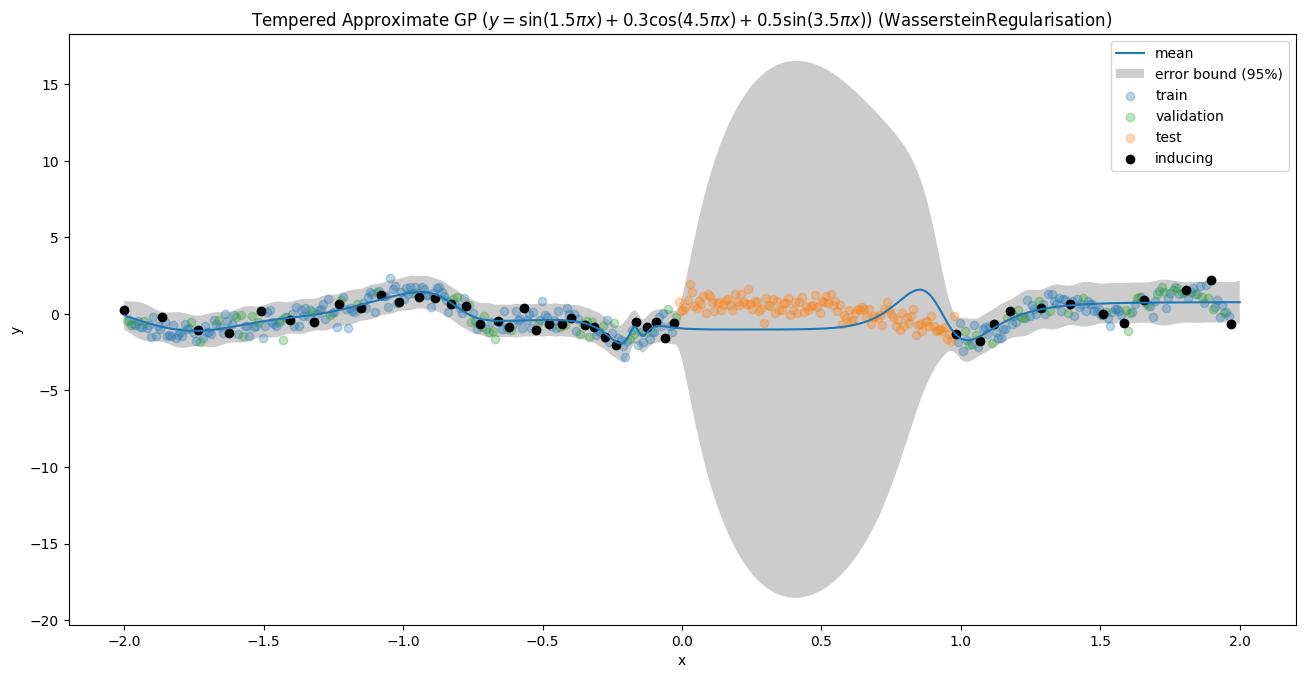
\includegraphics[width=0.9\linewidth]{experiments/regression/toy_curves/outputs/curve3/tempered-WassersteinRegularisation.png}
\end{minipage}%
\begin{minipage}{.5\textwidth}
  \centering
  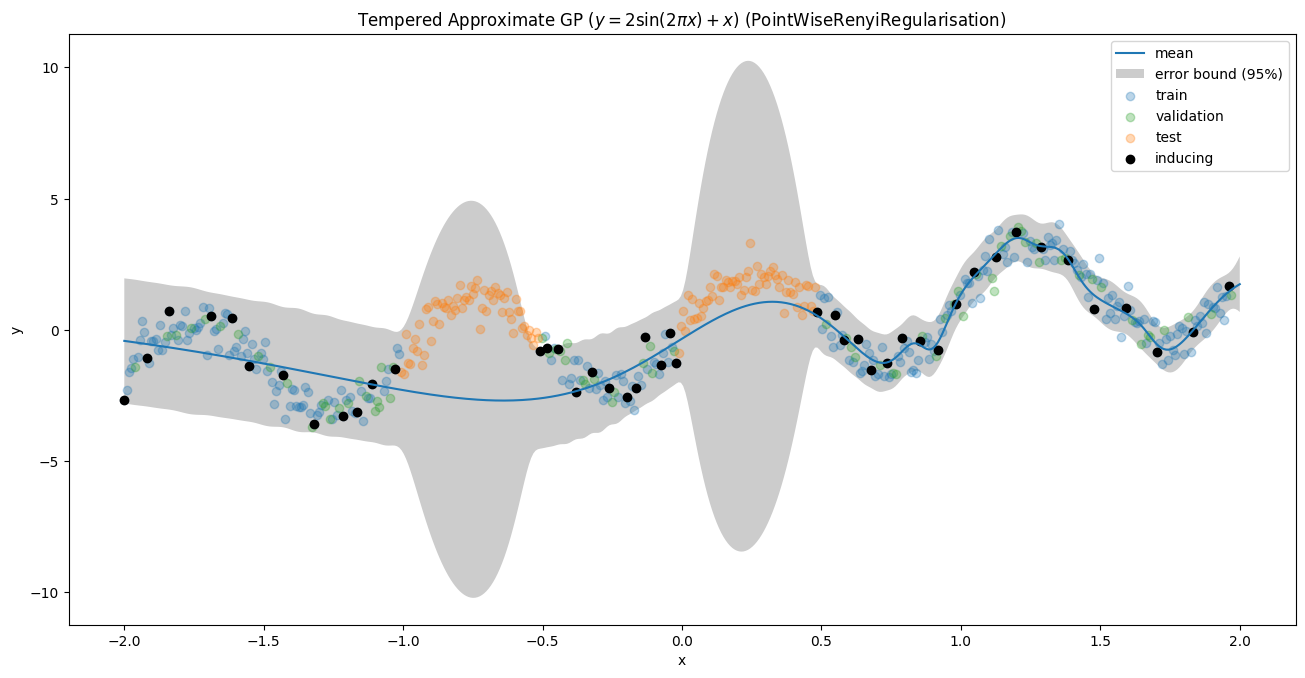
\includegraphics[width=0.9\linewidth]{experiments/regression/toy_curves/outputs/curve4/tempered-PointWiseRenyiRegularisation.png}
\end{minipage}
\caption{GVI-GPs for Regression}
\end{figure}
\subsection{Regression Results}

\subsection{Image Classification Results}

\newpage
\section{Future Work}
\subsection{NLP Named-Entity Recognition}

\newpage
\section{Conclusions}

\newpage
\bibliography{references}


\newpage
\appendix
\section{Appendix}

\subsection{KL Divergence and the Bayesian Posterior}\label{svgp-kld-bayesian}
We wish to match the log-likelihood of $P_{GP}$ for training data $\left\{ x_n, y_n\right\}$ by maximising the lower bound with respect to $\nu$ for $Q_{GP}^{\nu}$ on inducing points $\{x_m, y_m\}_{m=1}^{M}$. We begin by reformulating the log-likelihood:
\begin{align}
    \mathcal{L} &= \log P\left(\left\{ y_n\right\} \big\vert\left\{ x_n\right\}\right)
    \\&= \log P\left(\left\{ y_n\right\} \big\vert \mathbf{Y}_M, \left\{ x_m\right\}, \left\{ x_n\right\}\right)
    \\&= \log \int_{\mathbb{R}^M} P\left(\left\{ y_n\right\}, \mathbf{Y}_M \big\vert \left\{ x_m\right\}, \left\{ x_n\right\}\right) d\mathbf{Y}_M
\end{align}
Introducing $Q^{\nu}\left(\mathbf{Y}_M \big\vert \left\{ x_m\right\} \right)$, the $Q_{GP}^{\nu}$ prior on the inducing points, we can equivalently write:
\begin{align}
            \mathcal{L} &= \log \int_{\mathbb{R}^M} \frac{P\left(\left\{ y_n\right\}, \mathbf{Y}_M \big\vert \left\{ x_m\right\}, \left\{ x_n\right\}\right)Q^{\nu}\left(\mathbf{Y}_M \big\vert \left\{ x_m\right\} \right)}{Q^{\nu}\left(\mathbf{Y}_M \big\vert \left\{ x_m\right\} \right)} d\mathbf{Y}_M
    \\&= \log \int_{\mathbb{R}^M} \frac{P\left(\left\{ y_n\right\} \big\vert \mathbf{Y}_M , \left\{ x_m\right\}, \left\{ x_n\right\}\right)P\left(\mathbf{Y}_M \big\vert \left\{ x_m\right\}\right)Q^{\nu}\left(\mathbf{Y}_M \big\vert \left\{ x_m\right\} \right)}{Q^{\nu}\left(\mathbf{Y}_M \big\vert \left\{ x_m\right\} \right)} d\mathbf{Y}_M
    \\&\qquad\geq  \int_{\mathbb{R}^M} Q^{\nu}\left(\mathbf{Y}_M \big\vert \left\{ x_m\right\} \right) \log \left(\frac{P\left(\left\{ y_n\right\} \big\vert \mathbf{Y}_M , \left\{ x_m\right\}, \left\{ x_n\right\}\right)P\left(\mathbf{Y}_M \big\vert \left\{ x_m\right\}\right)}{Q^{\nu}\left(\mathbf{Y}_M \big\vert \left\{ x_m\right\} \right)} \right)d\mathbf{Y}_M
    \label{log-like-jensen}
    \\ & \qquad\qquad \eqqcolon \mathcal{L_{free}(\nu)}
\end{align}
where we lower bound the log-likelihood with Jensen's inequality in (\ref{log-like-jensen}). $\mathcal{L_{free}(\nu)}$ is the free energy or evidence lower bound (ELBO) and can be expressed:
\begin{multline}
    \mathcal{L_{free}(\nu)} = \int_{\mathbb{R}^M} Q^{\nu}\left(\mathbf{Y}_M \big\vert \left\{ x_m\right\} \right) \log P\left(\left\{ y_n\right\} \big\vert \mathbf{Y}_M , \left\{ x_m\right\}, \left\{ x_n\right\}\right)d\mathbf{Y}_M
    \\ + \int_{\mathbb{R}^M} Q^{\nu}\left(\mathbf{Y}_M \big\vert \left\{ x_m\right\} \right) \log \left(\frac{P\left(\mathbf{Y}_M \big\vert \left\{ x_m\right\}\right)}{Q^{\nu}\left(\mathbf{Y}_M \big\vert \left\{ x_m\right\} \right)} \right)d\mathbf{Y}_M
\end{multline}
Recovering the standard result:
\begin{align}
    \mathcal{L_{free}(\nu)} &=  \log P\left(\left\{ y_n\right\} \big\vert \left\{ x_n\right\}\right) - \KLD\left[Q^{\nu}\left(\mathbf{Y}_M \big\vert \left\{ x_m\right\} \right) \| P\left(\mathbf{Y}_M \big\vert \left\{ x_m\right\} \right)\right]
    \\ &= \sum_{n=1}^N \left[\log P \left(y_n \big\vert  x_n \right)\right] - \KLD\left[Q^{\nu}\left(\mathbf{Y}_M \vert \left\{ x_m\right\} \right) \| P\left(\mathbf{Y}_M \big\vert \left\{ x_m\right\} \right)\right]
\end{align}
We see from (\ref{log-like-jensen}) that $\mathcal{L_{free}(\nu)}$ can also be expressed:
\begin{align}
    \mathcal{L_{free}(\nu)} &= - \mathbb{E}_{\mathbf{Y}_M \sim Q^{\nu}\left(\mathbf{Y}_M \big\vert \left\{ x_m\right\} \right)} \left[\log \left(\frac{Q^{\nu}\left(\mathbf{Y}_M \big\vert \left\{ x_m\right\} \right)}{P\left(\left\{ y_n\right\} \big\vert \mathbf{Y}_M , \left\{ x_m\right\}, \left\{ x_n\right\}\right)P\left(\mathbf{Y}_M \big\vert \left\{ x_m\right\}\right)} \right) \right]\\
    &= -\KLD \left[Q^{\nu}\left(\mathbf{Y}_M \big\vert \left\{ x_m\right\} \right) \| P\left(\mathbf{Y}_M \big\vert \left\{ x_m\right\}, \left\{ y_n\right\}, \left\{ x_n\right\}\right) \right]
    \label{free-energy-kld}
\end{align}
where we see that $P\left(\mathbf{Y}_M \big\vert \left\{ x_m\right\}, \left\{ y_n\right\}, \left\{ x_n\right\}\right) \propto P\left(\left\{ y_n\right\} \big\vert \mathbf{Y}_M , \left\{ x_m\right\}, \left\{ x_n\right\}\right)P\left(\mathbf{Y}_M \big\vert \left\{ x_m\right\}\right)$, the posterior distribution.
Thus, the KL divergence is the natural divergence that arises from a Bayesian approach. (\ref{free-energy-kld}) is the negative KL between the prior of the approximating distribution $Q^{\nu}$ and the \textit{true} Bayesian posterior of $P$. In other words, $Q^{\nu*}$ is the projection of the Bayesian posterior onto the space of approximating GPs $\left\{Q^{\nu}: \nu \in \Gamma\right\}$ with respect to the KL divergence. This is indicated as the minimisation of the $\KLD$ in (\ref{svgp-minimiser}).

\subsection{Trace Kernel Proof for the NNGP Kernel}\label{svgp-kld-bayesian}
\end{document}